\chapter{移动界面问题虚单元方法及其在涡电流问题中的应用}
在本章中我们将前面章节使用的界面拟合网格方法和虚单元方法扩展到
抛物方方程的移动界面问题中。
我们首先介绍了使用的界面拟合网格生成算法,
该算法使用界面切割背景网格的方法,来高效生成拟合移动界面的网格。
随后我们给出了抛物方程的虚单元方法的基本原理以及具体的实现细节,
其中由于界面的移动,我们引入了一个中间网格来处理两个时间层之间函数的传递问题。
最后我们给出了数值算例验证方法的有效性。

\section{模型问题}
考虑如下的抛物型方程:
\begin{equation}
\label{parabolic}
\begin{aligned}
    \partial_t u - \nabla \cdot (\beta \nabla u) & = f, \quad \text{ in } \quad
    \Omega \times (0, T),\\
    u & = 0, \quad \text{ in } \quad \partial \Omega \times (0, T),\\
    u & = u_0, \quad \text{ in } \quad \Omega \times \{0\}.
\end{aligned}
\end{equation}
其中,$\Omega$ 是 $\mathbb{R}^2$ 中的有界区域,具有 Lipschitz 连续的边界
$\partial \Omega$,$T > 0$ 为最终时间,$f \in L^2([0, T], L^2(\Omega))$ 为源项,$u_0$
为初始条件。系数 $\beta$ 在 $\Omega$ 内是分段常数函数:
$$
\beta(t) = 
\begin{cases}
    \beta^+(t), & \text{ in } \quad \Omega^+(t),\\
    \beta^-(t), & \text{ in } \quad \Omega^-(t).
\end{cases}
$$
其中,$\Omega^+(t)$ 和 $\Omega^-(t)$ 是由随时间演化的界面 $\Gamma(t)$ 所分隔的两个子区域。函数 $u$ 在界面 $\Gamma(t)$ 上满足跳跃条件:
\begin{equation}
\begin{aligned}
    [u]|_{\Gamma(t)} = u^+|_{\Gamma(t)} - u^-|_{\Gamma(t)} = 0, \quad t\in (0, T),\\
    [\beta \frac{\partial u}{\partial \boldsymbol{n}}]|_{\Gamma(t)} =
    \beta^+\frac{\partial u^+}{\partial \boldsymbol{n}}|_{\Gamma(t)} 
    - 
    \beta^-\frac{\partial u^-}{\partial \boldsymbol{n}}|_{\Gamma(t)} = 0, \quad t\in (0, T),
\end{aligned}
\end{equation}
其中,$u^+$ 和 $u^-$ 分别表示 $u$ 在 $\Omega^+(t)$ 和 $\Omega^-(t)$
内的值,$\boldsymbol{n}$ 为界面 $\Gamma(t)$ 上从 $\Omega^-(t)$ 指向 $\Omega^+(t)$ 的单位法向量。

抛物型方程 \eqref{parabolic} 的弱形式为:求 $u \in L^2(0, T, H^1_0(\Omega))$ 且
$\partial_t u \in L^2(0, T, H^{-1}(\Omega))$,
使得
\begin{equation}
\label{weakform}
\begin{aligned}
    (\partial_t u, v) + a(u, v) & = (f, v), \quad \forall v \in H^1_0(\Omega),
\end{aligned}
\end{equation}
其中,
$$
a(u, v) = \int_{\Omega} \beta \nabla u \cdot \nabla v \,\mathrm{d}x.
$$
\section{虚单元空间}
本节给出问题 \eqref{weakform} 的虚单元离散格式,
本文仅考虑最低阶的虚单元空间,其已在第一章定义,为了完整性,我们在此再重申一遍。

设$\mathcal{T}_h$为区域$\Omega$上的多边形网格。
定义局部虚单元空间$V_h(K)$之前,
先定义一个比$V_h(K)$更大的局部空间$\tilde{V}_h(K)$:
\begin{align}
\tilde{V}_h(K) & := \{ v_h \in H^1(K) : ~ \Delta v_h \in \mathbb{P}_1(K); v_h|_e\in\mathbb{P}_1(e), ~ \forall e \in
\mathcal{E}(K) \},  
\label{biggervespace}
\end{align}

定义从$\tilde{V}_h(K)$到$\mathbb{P}_1(K)$的$H^1$投影算子$\Pi_K^1$:
\begin{equation}
\label{h1projection}
\begin{aligned}
(\nabla\Pi_K^1 v_h, \nabla q)_{K} & = (\nabla v_h, \nabla q)_{K}, \quad \forall
q \in \mathbb{P}_1(K),\\
P_0(\Pi_K^1 v_h) & = P_0(v_h).
\end{aligned}
\end{equation}
其中$P_0$是 $\tilde{V}_h$ 上的一个线性泛函,定义为$K$上所有顶点函数值的总和:
$$
P_0(v_h) = \sum_{\delta \in \mathcal{V}(K)} v_h (\delta).
$$
定义从$\tilde{V}_h(K)$到$\mathbb{P}_1(K)$的$L^2$投影算子$\Pi_K^0$:
$$
(\Pi_K^0 v_h, q)_{K} = (v_h, q)_{K}, \quad \forall q \in \mathbb{P}_1(K),
$$
于是局部虚单元空间$V_h(K)$定义为:
\begin{align}
    V_h(K) & = \{ v_h \in \tilde{V}_h(K) : ~ \Pi_K^1 v_h = \Pi_K^0 v_h \}.
\end{align}

在$V_h(K)$中的函数$v$可以由其在$K$的顶点值唯一确定:
$$
\mathrm{dof}_i^K(v) := v(\delta_i) \quad i = 1, 2, \dots, N_K, \quad \delta_i
\in \mathcal{V}(K),
$$
由于$\Pi_K^1 = \Pi_K^0$,
为简化符号表示,我们在$V_h(K)$上统一记$\Pi_K^1$和$\Pi_K^0$为$\Pi_K$。需要说明的是
$\Pi_K$可以通过自由度直接计算,具体形式见下一章 \ref{projectionmatrix}。

全局虚单元空间$V_h(\mathcal{T}_h)$定义为:
$$
V_h(\mathcal{T}_h) := \{ v_h \in H^1_0(\Omega) : ~ v_h|_K \in V_h(K), ~ \forall
K \in \mathcal{T}_h \},
$$
定义全局投影算子$\Pi_h : V_h(\mathcal{T}_h) \to 
\Pi_{K\in\mathcal{T}_h} \mathbb{P}_1(K)$,
满足对每个$K \in \mathcal{T}_h$均有$\Pi_h|_K = \Pi_K$。

\subsection{投影算子的矩阵形式}
\label{projectionmatrix}
投影算子$\Pi_K$是从$V_h(K)$到$\mathbb{P}_1(K)$的线性算子,在 
$V_h(K)$ 和 $\mathbb{P}_1(K)$ 中选择合适的基函数,根据
\eqref{h1projection} 式,可以得到投影算子的矩阵形式。

对于每个单元$K \in \mathcal{T}_h$,记$h_K$为$K$的直径,$(x_K,
y_K)$为$K$的重心,$\boldsymbol{n}_K$ 为定义在 
$\partial K$上的外法向单位向量。定义缩放单项式基$\mathcal{M}_1(K)
= \{m_{i}\}_{i=1}^3$:
$$
m_1 = 1, \quad m_2 = \frac{x - x_K}{h_K}, \quad m_3 = \frac{y - y_K}{h_K},
$$
其中$\mathcal{M}_1(K)$是$\mathbb{P}_1(K)$的一组基。
定义单元质量矩阵$\tilde{\boldsymbol{M}}_K$:
$$
(\tilde{\boldsymbol{M}}_K)_{ij} = (m_i, m_j)_K,
$$
以及单元刚度矩阵$\tilde{\boldsymbol{A}}_K$:
$$
\tilde{\boldsymbol{A}}_K =
\begin{pmatrix}
    (\nabla m_i, \nabla m_j)_K.
\end{pmatrix}_{3\times 3}
 =
\begin{pmatrix}
    0 & 0 & 0\\
    0 & \frac{|K|}{h_K^2} & 0\\
    0 & 0 & \frac{|K|}{h_K^2}
\end{pmatrix},
$$
其中$|K|$为单元$K$的面积。

定义标量多项式函数自由度矩阵$\boldsymbol{D}_K$:
$$
\boldsymbol{D}_K := (\mathrm{dof}_i^K(m_j))_{N_K\times 3},
$$
其满足:
$$
m_i = \sum_{j=1}^{N_K}(\boldsymbol{D}_K)_{ji}\phi_j.
$$
定义矩阵$\boldsymbol{G}_K$:
$$
\boldsymbol{G}_K =
\begin{pmatrix}
    P_0(m_1) & P_0(m_2) & P_0(m_3)\\
    0 & (\nabla m_2, \nabla m_2)_K & (\nabla m_2, \nabla m_3)_K\\
    0 & (\nabla m_3, \nabla m_2)_K & (\nabla m_3, \nabla m_3)_K
\end{pmatrix}
=
\begin{pmatrix}
    P_0(m_1) & P_0(m_2) & P_0(m_3)\\
    0 & \frac{|K|}{h_K^2} & 0\\
    0 & 0 & \frac{|K|}{h_K^2}
\end{pmatrix}.
$$
假设 \(\{\phi_i\}_{i=1}^{N_K}\) 是空间 \(V_h(K)\) 的一组基函数,并满足\( \mathrm{dof}_i^K(\phi_j) = \delta_{ij} \)。定义矩阵 \(\boldsymbol{B}_K\) 如下:
\[
\boldsymbol{B}_K =
\begin{pmatrix}
    P_0(\phi_1) & P_0(\phi_2) & \dots & P_0(\phi_{N_K})\\
    (\nabla m_2, \nabla \phi_1)_K & (\nabla m_2, \nabla \phi_2)_K & \dots & (\nabla m_2, \nabla \phi_{N_K})_K\\
    (\nabla m_3, \nabla \phi_1)_K & (\nabla m_3, \nabla \phi_2)_K & \dots & (\nabla m_3, \nabla \phi_{N_K})_K
\end{pmatrix},
\]
其中
\[
\begin{aligned}
P_0(\phi_i) &= 1, \quad i = 1, 2, \dots, N_K, \\
(\nabla m_j, \nabla \phi_i)_K &= \int_{\partial K} \frac{\partial m_j}{\partial \boldsymbol{n}}\phi_i \,\mathrm{d} s,\quad i = 1, 2, \dots, N_K, \quad j = 2, 3.
\end{aligned}
\]
矩阵 \(\boldsymbol{B}_K\) 可以通过基函数 \(\phi_i\) 的自由度计算得到。

设 \(\boldsymbol{\Pi}_K\) 为投影算子 \(\Pi_K\) 的矩阵形式,即
\[
\Pi_K \phi_i = \sum_{j=1}^{3} (\boldsymbol{\Pi}_K)_{ji} m_j.
\]
将其代入 \ref{h1projection} 中 $\Pi_K$ 的定义,我们得到
$$
\boldsymbol{\Pi}_K = \boldsymbol{G}_K^{-1} \boldsymbol{B}_K.
$$
事实上,$\mathbb{P}_1(K)$ 是 $V_h(K)$ 的一个子空间,因此 $\Pi_K$ 
也可认为是一个从 $V_h(K)$ 到 $V_h(K)$ 的投影算子。
定义矩阵 $\boldsymbol{\Pi}_K^* = \boldsymbol{D}_K \boldsymbol{\Pi}_K$,显然其满足:
$$
\Pi_K \phi_i = \sum_{j=1}^{N_K} (\boldsymbol{\Pi}_K^*)_{ji} \phi_j, \quad i = 1,
2, \dots, N_K,
$$
即 $\boldsymbol{\Pi}_K^*$ 就是 $\Pi_K : V_h(K) \to V_h(K)$ 的矩阵形式。

\section{带有移动界面的抛物方程虚单元方法}
\label{vemformulation}
在本节中,我们介绍用于求解抛物方程 \eqref{parabolic} 的虚单元方法,并提供具体的实现细节。

\subsection{界面网格生成}
\label{meshgeneration}
首先我们给出了一种高效且便捷的界面拟合网格生成算法。
为了精确描述角点信息,我们使用离散点列来表示界面。对于界面
$\Gamma$,将其离散化为点集 $\{\boldsymbol{p}_0, \boldsymbol{p}_1, \dots,
\boldsymbol{p}_{n-1}\}$,其中包含界面上的角点。令 $\boldsymbol{p}_n =
\boldsymbol{p}_0$,然后依次用直线连接相邻点对 $(\boldsymbol{p}_i,
\boldsymbol{p}_{i+1})$,其中 $i = 0, 1, \dots,
n-1$,从而得到界面的近似表示,记作 $\tilde{\Gamma}$。假设在区域 $\Omega$
上已有一个背景网格 $\mathcal{T}_h^b$,则网格生成算法如下:

\begin{itemize}
    \item[1.] 计算所有直线段 $(\boldsymbol{p}_i, \boldsymbol{p}_{i+1}) \in
        \tilde{\Gamma}$ 与背景网格 $\mathcal{T}_h^b$ 边的交点。记距离
        $\boldsymbol{p}_i$ 最近的两个交点为 $\boldsymbol{p}^0_i$ 和
        $\boldsymbol{p}^1_i$,按顺序将所有交点存入点集 $V^I$。
    \item[2.] 点集 $V^I$ 中相邻的两个点必定位于同一单元的边上,
        连接这两个点即可将该单元划分为两个子单元。
    \item[3.] 交点 $\boldsymbol{p}^0_i$ 和 $\boldsymbol{p}^1_i$
        必定在 $V^I$ 中相邻,因此在上一步骤中已将其连接成网格边,
        记作 $e_i$。如果
        $\boldsymbol{p}_i$ 是角点,则在 $e_i$ 的中心点添加一个新节点,将 $e_i$
        划分为两个子边,并将该中心点移动到 $\boldsymbol{p}_i$。
\end{itemize}
该算法的基本思想是直接利用界面对背景网格进行裁剪,生成过程如图
\ref{fig:UnfitMesh} 所示。

\begin{figure}[h]
\centering
\begin{subfigure}{.24\textwidth}
    \centering
    \includegraphics[width=1.3in]{./figures/movingmaxwell/interface_half_cricle.pdf}
    \label{fig:UnfitMesh1} %% label for first subfigure
\end{subfigure}
%%
\begin{subfigure}{.24\textwidth}
    \centering
    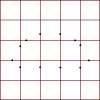
\includegraphics[width=1.3in]{./figures/movingmaxwell/cut_point.pdf}
    \label{fig:UnfitMesh2} %% label for first subfigure
\end{subfigure}
\begin{subfigure}{.24\textwidth}
    \centering
    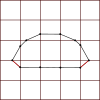
\includegraphics[width=1.3in]{./figures/movingmaxwell/cut_mesh_0.pdf}
    \label{fig:NonConfMesh1} %% label for first subfigure
\end{subfigure}
%%
\begin{subfigure}{.24\textwidth}
    \centering
    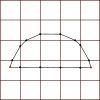
\includegraphics[width=1.3in]{./figures/movingmaxwell/cut_mesh_1.pdf}
    \label{fig:NonConfMesh2} %% label for first subfigure
\end{subfigure}
\caption{界面拟合网格生成算法:第一张图为背景网格与半圆形界面,界面被离散为
12 个点,第二张图展示了界面与背景网格的交点 $V^I$,第三张图为以此连接交点,
第四张图为处理角点的情况.}
\label{fig:UnfitMesh}
\end{figure}

\subsection{空间离散}
设 $\mathcal{T}_h^b$ 为定义在区域 $\Omega$ 上的背景网格,$\Gamma^t$ 表示时刻 $t$
的界面,$\mathcal{T}_h^t$ 为算法 \ref{meshgeneration} 生成的 $\Omega^{\pm}$
的网格,$V_h^t$ 为定义在 $\mathcal{T}_h^t$ 上的虚单元空间。
\eqref{weakform} 式的虚单元离散格式为:求 $u_h(\cdot, t) \in V_h^t$,使得
\begin{equation}
\label{vem}
(\partial_t u_h, \Pi_h v_h) + a_h(u_h, v_h) = (f, \Pi_h v_h), \quad \forall v_h
\in V_h^t,
\end{equation}
其中
\begin{align}
    a_h(u_h, v_h) & := \sum_{K\in \mathcal{T}_h^t} a_K(u_h, v_h), \\
    a_K(u_h, v_h) & := (\beta\nabla \Pi_K u_h, \nabla \Pi_K v_h)_{K}
    + S_K( (I-\Pi_K) u_h, (I-\Pi_k)v_h),
\end{align}
其中 $S_K$ 是稳定化项,在第 4 章中已讨论过去除了稳定化项 $S_K$ 的方法,
这是仍然使用标准虚单元方法进行离散。$S_K$ 的定义如下:
$$
S_K(u_h, v_h) := \sum_{i = 0}^{N_K} \text{dof}_i(u_h) \text{dof}_i(v_h).
$$
这种稳定化项称为 dof-dof 型稳定化项。%有其他类型的稳定化项可参考\CC{文献文献文献}。

\subsection{时间离散}
\label{timediscretization}
现在,我们对涡电流方程的时间离散化采用向后欧拉方法。
将时间区间 $[0, T]$ 划分为 $N$ 个子区间,时间步长为 $\tau = T/N$,令 $t^n =
n\tau, n = 0, 1, \dots, N$。为了简化表示,定义函数 $u^n(\boldsymbol{x}) =
u(\boldsymbol{x}, t^n)$,虚单元空间记作 $V_h^n = V_h(t^n)$,$L^2$ 投影算子在 $V_h^n$ 上为 $\Pi_h^n$,在上下文清晰时,我们省略其上标 $n$。
定义向后差分算子:
$$
\delta_t u_h^n := \frac{\Pi_h^nu_h^n - \Pi_h^{n-1} u_h^{n-1}}{\tau}.
$$
将方程 \eqref{vem} 中的时间导数替换为向后差分算子,我们得到如下离散问题:
求解 $u_h^n \in V_h^n$ 使得:
\begin{equation}
\label{VEMdiscrete}
(\delta_t u_h^n, \Pi_h v_h) + a_h(u_h^n, v_h) = (f^n,\Pi_h v_h),
\quad \forall v_h \in V_h^n.
\end{equation}
对上式重新排列,我们得到:
\begin{equation}
\label{VEMdiscrete2}
\frac{1}{\tau}( \Pi_h u_h^n,\Pi_h v_h) + a_h(u_h^n, v_h) =
(f^n, \Pi_h v_h) + \frac{1}{\tau}(\Pi_h u_h^{n-1},\Pi_h v_h)
\quad \forall v_h \in V_h^n.
\end{equation}
需要注意的是,在项 $\frac{1}{\tau}( \Pi_h u_h^{n-1}, \Pi_h v_h)$ 中,$\Pi_h u_h^{n-1}$ 是定义在网格 $\mathcal{T}_h^{n-1}$ 上,而 $v_h$ 是定义在网格 $\mathcal{T}_h^n$ 上,因此该项无法直接计算。

在有限元方法中,通常的做法是将 $u_h^{n-1}$ 插值到网格
$\mathcal{T}_h^n$,但这种处理会引入额外的插值误差,特别是在 $\Pi_h u_h^{n-1}$
在边界附近变化剧烈的情况下。然而,在虚单元方法中,插值并不是必须的。下面我们提出一种方法,以避免在上述框架下进行插值。

\subsection{中间网格}
考虑一个简化的情况,假设背景网格是一个正方形单元
$K$,且移动的界面是一个直线,网格$\mathcal{T}_h^{n-1}$和$\mathcal{T}_h^n$如图\ref{fig:overlapmesh}所示,四边形$K$由$\Gamma^{n-1}$和$\Gamma^n$切分成$K_1^{n-1}$、$K_2^{n-1}$和$K_1^n$、$K_2^n$两个部分。

%图片
\begin{figure}[h]
    \centering
    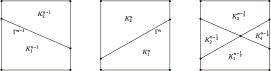
\includegraphics[width=4in]{./figures/movingmaxwell/overlap_interface.pdf}
    % \caption{Type I:5 tetrahedra}
    \caption{单元分别被 $\Gamma^{n-1}$、$\Gamma_h^n$ 和
    $\Gamma^{n}\cup\Gamma^{n-1}$切割.}
     \label{fig:overlapmesh} %% label for first subfigure
\end{figure}

假设函数$u_h^{n-1}\in V_h^{n-1}$定义在网格$\mathcal{T}_h^{n-1}$上,
函数$v_h\in V_h^{n}$定义在网格$\mathcal{T}_h^n$上,我们知道:
\begin{itemize}
    \item $\Pi_h
        u_h^{n-1}$在$K_1^{n-1},K_2^{n-1}$上是多项式,但在$K_1^n$和$K_2^n$上不是多项式。
    \item $\Pi_h
        v_h$在$K_1^n$和$K_2^n$上是多项式,但在$K_1^{n-1}$和$K_2^{n-1}$上不是多项式。
\end{itemize}
因此,我们无法直接计算$(\Pi_h u_h^{n-1}, \Pi_h v_h)_K$这一项。
为了解决这个问题,我们引入一个中间网格$\mathcal{T}_h^{n-1/2}$,该网格是通过用界面$\Gamma^{n-1}\cup\Gamma^n$切割四边形$K$得到的。然后,四边形$K$被分割为四个子四边形$K_1^{n-1/2}$、$K_2^{n-1/2}$、$K_3^{n-1/2}$和$K_4^{n-1/2}$,如图\ref{fig:overlapmesh}所示,并且$\Pi_h
u_h^{n-1}$和$\Pi_h
v_h$是这些四个子四边形上的多项式函数。这样,我们可以通过以下公式来计算$(\Pi_h
u_h^{n-1}, v_h)_K$:
$$
\begin{aligned}
    (\Pi_h u_h^{n-1}, \Pi_h v_h)_K =
    &
    (\Pi_{K_1^{n-1}}u_h^{n-1}, \Pi_{K_1^{n}}v_h)_{K_1^{n-1/2}}
    +
    (\Pi_{K_1^{n-1}}u_h^{n-1}, \Pi_{K_2^{n}}v_h)_{K_2^{n-1/2}}\\
    & +
    (\Pi_{K_2^{n-1}}u_h^{n-1}, \Pi_{K_2^{n}}v_h)_{K_3^{n-1/2}}
    +
    (\Pi_{K_2^{n-1}}u_h^{n-1}, \Pi_{K_1^{n}}v_h)_{K_4^{n-1/2}}.
\end{aligned}
$$

实际上,上述公式对一般网格也是成立的。
对于一般情况,同样地,我们用界面$\Gamma^{n-1}\cup\Gamma^n$切割背景网格得到
中间网格$\mathcal{T}_h^{n-1/2}$,
那么$\mathcal{T}_h^{n-1/2}$是网格$\mathcal{T}_h^{n-1}$
和$\mathcal{T}_h^n$的共同子网格。
然后我们可以使用以下公式来计算$(\Pi_h u_h^{n-1}, \Pi_h v_h)$:
\begin{equation}
\label{inner_product_of_two_layer_basis}
(\Pi_h u_h^{n-1}, \Pi_h v_h) = \sum_{K\in \mathcal{T}_h^{n-1/2}}
(\Pi_{K^{n-1}}u_h^{n-1}, \Pi_{K^n}v_h)_{K}.
\end{equation}
其中$K^{n}$和$K^{n-1}$分别是网格$\mathcal{T}_h^n$和$\mathcal{T}_h^{n-1}$上$K$的父单元,如图\ref{fig:parentelement}所示。
这样我们就做到了不需要插值就可以计算$(\Pi_h u_h^{n-1}, \Pi_h v_h)$。

% 图片
\begin{figure}[h]
\centering
%%%%%
\begin{subfigure}{.3\textwidth}
    \centering
    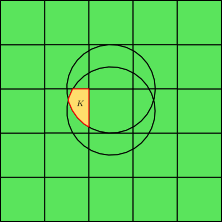
\includegraphics[width=1.5in]{./figures/movingmaxwell/meshncut.pdf}
\end{subfigure}
%%
\begin{subfigure}{.3\textwidth}
    \centering
    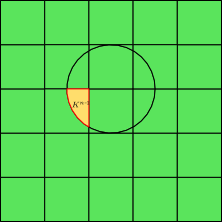
\includegraphics[width=1.5in]{./figures/movingmaxwell/meshn_1.pdf}
\end{subfigure}
%%
\begin{subfigure}{.3\textwidth}
    \centering
     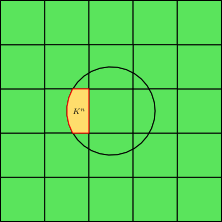
\includegraphics[width=1.5in]{./figures/movingmaxwell/meshn.pdf}
\end{subfigure}
\caption{一个界面从上到下移动的圆形,背景网格是一个$5\times5$的正方形网格,
    从左到右的三张图分别是网格$\mathcal{T}_h^{n-1/2}$、
    $\mathcal{T}_h^{n-1}$和$\mathcal{T}_h^{n}$,其中单元$K^n$和$K^{n-1}$是$K$的父单元.}
  \label{fig:parentelement} %% label for entire figure
\end{figure}

\subsection{矩阵形式与算法}
\label{matrixformulation}
设$\{\phi_i\}_{i=1}^{N^n}$为$V_h(\mathcal{T}^n_h)$的基,
$N^n$为$V_h(\mathcal{T}^n_h)$的维数,向量$\boldsymbol{U}^n
= (U^n_1, \dots, U^n_{N^n})$为$u_h^n$的自由度,即$u_h^n = \sum_{i=1}^{N^n} U^n_i
\phi_i$,则方程\eqref{VEMdiscrete2}可以写成如下形式:
\begin{equation}
\label{matrixform}
\frac{1}{\tau}\boldsymbol{M}^n \boldsymbol{U}^n + \boldsymbol{A}^n \boldsymbol{U}^n =
\boldsymbol{F}^n + \frac{1}{\tau}\boldsymbol{R}^n,
\end{equation}
其中
$$
\begin{aligned}
(\boldsymbol{M}^n)_{ij} & = (\Pi_h \phi_i, \Pi_h \phi_j)_{\Omega},\\
(\boldsymbol{A}^n)_{ij} & = a_h(\phi_i, \phi_j),\\
(\boldsymbol{F}^n)_i & = (f^n, \Pi_h \phi_i)_{\Omega},\\
(\boldsymbol{R}^n)_i & = (\Pi_h u_h^{n-1}, \Pi_h \phi_i)_{\Omega}.
\end{aligned}
$$
% 这些矩阵和向量的计算可以通过局部矩阵和向量计算得到
上述矩阵和向量可以通过在每个单元$K \in \mathcal{T}_h^n$上求和局部矩阵和向量来组装,因此,主要任务是计算局部矩阵和向量。

对于每个单元$K \in \mathcal{T}_h^n$,
根据第 \ref{projectionmatrix}
节中的投影算子的矩阵形式,我们可以得到缩放单项式的质量矩阵 $\tilde{\bM}_K$
、刚度矩阵 $\tilde{\bA}_K$ 自由度矩阵 $\bD_K$以及投影算子的两个矩阵
形式 $\bPi_K$ 和 $\bPi_K^*$。\eqref{matrixform} 式中的局部矩阵和向量将由
这些矩阵计算得到。

设$\{\phi_i\}_{i=1}^{N_K}$为$V_h(K)$的基,局部质量矩阵$\boldsymbol{M}_K$为:
$$
\boldsymbol{M}_K := ((\Pi_K \phi_i, \Pi_K \phi_j)_K)_{N_K\times N_K} =
\boldsymbol{\Pi}_K^T \tilde{\boldsymbol{M}}_K \boldsymbol{\Pi}_K,
$$
稳定化项矩阵$\boldsymbol{S}_K$为:
$$
\boldsymbol{S}_K := (S_K(\phi_i, \phi_j))_{N_K\times N_K} =
(\boldsymbol{I}-\boldsymbol{\Pi}_K^*)^T 
(\boldsymbol{I}-\boldsymbol{\Pi}_K^*),
$$
局部矩阵$\boldsymbol{A}_K$为:
$$
\boldsymbol{A}_K := (a_K(\phi_i, \phi_j))_{N_K\times N_K} =
\beta\boldsymbol{\Pi}_K^T \boldsymbol{\tilde{A}}_K \boldsymbol{\Pi}_K +
\boldsymbol{S}_K.
$$
局部向量$\boldsymbol{F}_K$为:
$$
(\boldsymbol{F}_K)_i := (f^n, \Pi_K \phi_i)_K =
\sum_{j=1}^3 \Pi_{ji}(f^n, m_j)_K,
$$
局部向量$\boldsymbol{R}_K$为:
$$
(\boldsymbol{R}_K)_i := (\Pi_K u_h^{n-1}, \Pi_K \phi_i)_K.
$$
该项可以通过公式\ref{inner_product_of_two_layer_basis}计算得到。

下面我们给出求解具有移动界面的抛物型方程的虚单元方法的算法流程。
\begin{algorithm}[H]
\caption{具有移动界面的抛物型方程的虚单元方法.}
\begin{algorithmic}[1]
\State 在计算区域$\Omega$ 上生成背景网格$\mathcal{T}_h^b$。
\State 在网格$\mathcal{T}_h^b$上建立虚单元空间$V_h^b$,并计算局部矩阵
    $\boldsymbol{M}_K, \boldsymbol{A}_K, \boldsymbol{\Pi}_K$。
\State 通过用界面$\Gamma^0$切割背景网格生成初始网格$\mathcal{T}_h^0$。
\State 将初值$u_0$插值到$V_h^0$上,得到$u_h^0$。
\For{$n = 1, 2, \dots, N$}
\State 更新界面,得到$\Gamma^{n}$。
\State 通过用界面$\Gamma^n, \Gamma^{n-1}\cup\Gamma^n$切割背景网格生成网格$\mathcal{T}_h^n, \mathcal{T}_h^{n-1/2}$。
\State 在$\mathcal{T}_h^n$上建立虚单元空间$V_h^n$。
\State 计算每个单元$K \in \{E \in \mathcal{T}_h^n: E \textrm{ 与 } \Gamma^n \textrm{相邻}\}$的局部矩阵
    $\boldsymbol{\Pi}_K, \boldsymbol{M}_K, \boldsymbol{A}_K$。
\State 计算每个单元$K \in \mathcal{T}_h^n$的局部向量
    $\boldsymbol{F}_K, \boldsymbol{R}_K$。
\State 组装全局矩阵和向量$\boldsymbol{M}^n, \boldsymbol{A}^n, \boldsymbol{F}^n, \boldsymbol{R}^n$。
\State 求解线性系统\eqref{matrixform},得到$\boldsymbol{U}^n$。
\EndFor
\end{algorithmic}
\end{algorithm}
\begin{remark}
    由于远离界面$\Gamma^n$的单元上的矩阵与 $\mathcal{T}_h^b$ 上的矩阵相同,
    因此我们只需要计算与界面$\Gamma^n$相邻的单元$K$的矩阵,
    这可以节省大量的计算时间。
\end{remark}

\section{轴对称涡电流方程的虚单元方法}
涡电流方程出现在许多工程应用中,例如电磁加热、
电磁成形等。在这些实际应用中,通常需要涉及到工件发生位移或变形,
因此需要考虑移动界面的影响。本节给出以磁矢势为未知量
的轴对称涡电流方程,该方程是一个抛物型方程,
我们将上一节的虚单元方法应用到该问题的模拟中。

\subsection{涡电流模型}
设$\Omega$为 $\mathbb{R}^3$ 中的单连通区域,考虑麦克斯韦方程组:
$$
\left\{
\begin{aligned}
  \bcurl \boldsymbol{H} & = \partial_t \boldsymbol{D} +
  \boldsymbol{J} \quad \quad & \text{Maxwell-Amp\'ere 方程,} \\
  \bcurl \boldsymbol{E} & = -\partial_t \boldsymbol{B}
  & \text{Faraday 方程,} \\
  \nabla\cdot \boldsymbol{D} & = \rho & \text{Gauss 电场方程,} \\
  \nabla\cdot \boldsymbol{B} & = 0 & \text{Gauss 磁场方程,}
\end{aligned}
\right.
$$
其中,$\boldsymbol{H}$是磁场,$\boldsymbol{E}$是电场,$\boldsymbol{B}$是磁通密度,$\boldsymbol{D}$是电通量密度,$\boldsymbol{J}$是电流密度,$\rho$是电荷密度。

根据法拉第定律, 变化的磁场在导体中会产生涡电流.
在很多实际应用中,电磁波的波长远远大于计算区域的直径,
此时可以认为电磁波的传播速度为 “无穷大”,电场和磁场的变化很慢,因此可以忽略
Maxwell 方程中 $\partial_t \boldsymbol{D}$,从而得到涡电流方程:
\begin{equation}
    \label{eddyeq}
    \bcurl \boldsymbol{H} = \boldsymbol{J}, \quad
    \bcurl \boldsymbol{E} = -\partial_t \boldsymbol{B}, \quad
    \nabla\cdot \boldsymbol{B} = 0.
\end{equation}

将$\Omega$划分为磁性区域$\Omega_{m}$、
线圈区域$\Omega_{c}$,导体区域$\Omega_{s}$
和空气区域$\Omega_{a}$,在不同材料的交界面$\Gamma$上满足以下条件:
$$
[\![\boldsymbol{H}\times \boldsymbol{n}]\!]_{\Gamma} = \boldsymbol{0}.
$$
根据欧姆定律和连续性方程,$\boldsymbol{B}$和$\boldsymbol{J}$满足:
\begin{equation}
\label{continuityBeq}
\boldsymbol{B} = \mu (\boldsymbol{H} + \boldsymbol{M}),
\end{equation}
\begin{equation}
\label{continuityJeq}
\boldsymbol{J} = \sigma(\boldsymbol{E}+\boldsymbol{u}\times \boldsymbol{B}) +
\boldsymbol{J}_s,
\end{equation}
其中,$\mu$是磁导率,$\boldsymbol{M}$是磁化强度,$\sigma$是电导率,
$\boldsymbol{u}$是$\Omega$上的速度场,$\boldsymbol{J}_s$是外加电流。
这些参数在不同区域有不同的值,特别地,在非磁性区域$\boldsymbol{M}
= 0$,在非导体区域$\sigma = 0$,在非线圈区域$\boldsymbol{J}_s = 0$。
不同区域中的电流 $\bJ$ 为:
$$
\boldsymbol{J} = \left\{
\begin{aligned}
    & \sigma (\bE + \bu\times \bB), \quad \text{导体区域(未知)}, \\
    & \boldsymbol{J}_s, \quad \text{线圈区域(外加电流,已知)}, \\
    & \boldsymbol{0}, \quad \text{其他区域}.
\end{aligned}
\right.
$$
因为 $\nabla\cdot\boldsymbol{B} = 0$, 所以存在向量场 $\boldsymbol{A}$ 满足 
$$
\boldsymbol{B} = \bcurl \boldsymbol{A}, 
$$
且满足库伦规范 $\diver \boldsymbol{A} = 0$, 我们称 $\boldsymbol{A}$
为磁矢势,根据法拉第方程有:
$$
\boldsymbol{E} = -\partial_t \boldsymbol{A}.
$$
这样根据 \eqref{eddyeq} 可以得到以磁矢势 $\bA$ 为未知量的
抛物型
涡电流方程:
\begin{equation}
    \label{vortexcurrent}
\sigma\partial_t \boldsymbol{A}+\bcurl(\frac{1}{\mu}\bcurl \boldsymbol{A}) 
- \sigma\boldsymbol{u}\times (\bcurl\boldsymbol{A})= \boldsymbol{J}_s + \bcurl
\boldsymbol{M}.
\end{equation}

\subsection{轴对称情况下的涡电流模型}
设 $\boldsymbol{e}_r$,$\boldsymbol{e}_\theta$,$\boldsymbol{e}_z$ 为
圆柱坐标系的基向量。假设我们的计算区域是一个圆柱体 $\Omega^{c} 
= \{(r, \theta, z):
0\leq r\leq R, 0\leq z\leq L\}$,其中 $R$ 是圆柱体的半径,$L$ 是圆柱体的高度。
$\Omega$ 是 $\Omega^{c}$ 与 $rz$ 平面的交集,即 $\Omega = \{(r, z):
0\leq r\leq R, 0\leq z\leq L\}$,如图\ref{fig:rzplane}所示。
\begin{figure}[htpb]
  \centering
  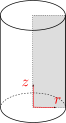
\includegraphics[width=0.15\textwidth]{./figures/movingmaxwell/rzplane.pdf}
  \caption{圆柱坐标系下 $rz$ 平面.}
  \label{fig:rzplane}
\end{figure}
考虑轴对称情况:
$\boldsymbol{A} = A(r, z) \boldsymbol{e}_\theta, \bJ_s = J_s(r, z) \be_{\theta}$,
其他变量不依赖于 $\theta$。
此时
$$
\bcurl \bA = -\frac{\partial A}{\partial z} \be_r + \frac{1}{r}
\frac{\partial (rA)}{\partial r} \be_z = - \frac{\partial A}{\partial
z} \be_r + (\frac{1}{r}A + \frac{\partial A}{\partial r}) \be_z.
$$
且对于任意两个函数 $f(r, z)$ 和 $g(r, z)$,其 $L^2$ 内积为:
\begin{equation}
\label{innerproduct}    
(f, g) = 2\pi\int_{\Omega} f(r, z) g(r, z) r dr dz.
\end{equation}
定义权重 Sobolev 空间:
$$
\begin{aligned}
L^2_r(\Omega) & := \{v \in L^2(\Omega): \int_{\Omega} |v(r, z)|^2 r dr dz <
\infty\},\\
H^1_r(\Omega) & := \{v \in H^1(\Omega): v \in L^2_r(\Omega), \nabla v \in 
L^2(\Omega, \mathbb{R}^2)\}.
\end{aligned}
$$
根据文献 \cite{Bermudez2013} 中的定义,我们知道 $A\be_\theta \in H(\bcurl;
\Omega^c)$ 当且仅当 $A \in \mathcal{V} := H^1_r(\Omega)\cap L^2_{1/r}(\Omega)$,
在轴对称情况下,涡电流方程对应的
变分问题为:求 $A \in L^2(0, T, \mathcal{V})$ 且 $\partial_t A \in L^2_r(0, T,
L^2(\Omega))$,使得
$\forall v \in \mathcal{V}, t \in [0, T]$ 有
$$
(\sigma\partial_t A, v) +
(\mu^{-1}\bcurl A\be_{\theta}, \bcurl v\be_{\theta}) =
(\sigma\boldsymbol{u}\times \bcurl A\be_{\theta} + J_s\be_{\theta}, v\be_{\theta}) 
+ (\boldsymbol{M}, \bcurl v\be_{\theta}).
$$
其中 $(\cdot, \cdot)$ 为\eqref{innerproduct}中定义的
$L^2$ 内积。
\subsection{轴对称涡电流方程的虚单元方法}
根据上述讨论,我们使用类似于第\ref{timediscretization}
节中的虚单元方法来求解轴对称涡电流方程。
将 $[0, T]$ 时间区间划分为 $N$ 个子区间,时间步长为 $\tau = T/N$,第
$n$ 个时间层的虚单元问题为:求 $A_h^n \in V_h$ 使得 
$\forall v_h \in V_h$ 有
\begin{equation}
\label{vemaxial}
\begin{aligned}
\frac{1}{\tau}
(\Pi_h A_h^n, v_h) + 
a_h(A_h^n, v_h) = (\sigma\bu\times \bcurl A_h^{n-1} \be_{\theta} +
    J_s\be_{\theta}, v_h\be_{\theta}) \\+ 
(\boldsymbol{M}, \bcurl v_h\be_{\theta})
+ \frac{1}{\tau}(\Pi_h A_h^{n-1}, v_h),
\end{aligned}
\end{equation}
其中
$$
\begin{aligned}
    a_h(A_h^n, v_h) & = \sum_{K\in \mathcal{T}_h} a_K(A^n_h, v_h),\\
    a_K(A^n_h, v_h) & = 2\pi\int_{K} \mu^{-1}\bcurl
\Pi_K A_h^n\be_{\theta}\cdot\bcurl v_h\be_{\theta} r \dd r \dd z
+ r_KS_K((I-\Pi_K)A_h^n, (I-\Pi_K)v_h),
\end{aligned}
$$
其中 $r_K$ 是单元 $K$ 重心的 $r$ 坐标,用以模拟 $L^2$ 内积
\eqref{innerproduct} 中的 $r$ 权重。
求解该问题的矩阵形式与算法与第\ref{matrixformulation}节中的类似,这里不再赘述。

\section{数值实验}
在本节中,我们展示了一些数值算例,以证明提出的方法的有效性。%
第一个数值实验是一个圆形界面的抛物方程移动界面问题,用于测试
方法的收敛性。在第二个算例中我们模拟了圆柱形磁体自由下落进入铜管的过程,
该过程基于轴对称涡电流方程建模。
所有实验都基于 FEALPy 软件库\cite{fealpy},在一台配备AMD
Ryzen 5 3500U CPU和64位Ubuntu 22.04操作系统的 PC 上实现。

\subsection{收敛性验证}
\label{sec:circle_interface}
在此算例中,我们考虑带有移动圆形界面的抛物型方程。区域为$\Omega = (0,1) \times
(0,1)$,圆形界面为$\Gamma(t) = \{(x,y)\in \Omega: (x-0.5)^2 + (y-0.7+0.2t)^2 =
R^2\}$,如图\ref{fig:circle_interface}所示,其中$R=0.2$。
真解为:
\begin{equation}
  u(x,y,t) = \left\{
    \begin{matrix}
        \frac{r^3(x, y, t)}{\beta_0}, &  r(x, y, t) < R,\\
        \frac{r^3(x, y, t)}{\beta_1} + \left(\frac{1}{\beta_0} -
        \frac{1}{\beta_1}\right)R^3, & \text{ 其它 }.
    \end{matrix}
    \right.
\end{equation}
其中$r(x, y, t) = \sqrt{(x-0.5)^2 + (y-0.7+0.2t)^2}$,$\beta_0 = 1$,$\beta_1 = 100$。源项$f(x,y,t)$由真解计算得到。

% t=0 时刻和 t=1 时刻的界面
\begin{figure}[H]
    \begin{minipage}[t]{0.49\linewidth}
        \centering
        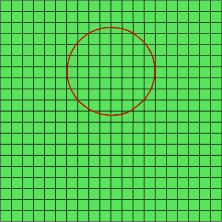
\includegraphics[width=0.5\textwidth]{./figures/movingmaxwell/circle_interface_0.pdf}
    \end{minipage}
    \begin{minipage}[t]{0.49\linewidth}
        \centering
        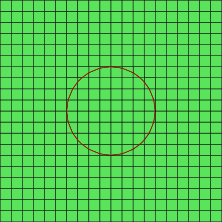
\includegraphics[width=0.5\textwidth]{./figures/movingmaxwell/circle_interface_1.pdf}
    \end{minipage}
    \caption{计算区域和 $t=0$(左)、$t=1$(右)时界面位置以及界面拟合网格示意图.}
    \label{fig:circle_interface}
\end{figure}

表\ref{tab:circle_interface}展示了 $t = 1$ 时刻的数值解的误差和收敛阶。
可以看到,
$$
\|u-\Pi_h u_h\|_{\Omega} = o(h^2), \quad \|u - u_h\|_{\infty,\Omega} = o(h^2),
\quad \|\nabla u-\nabla_h \Pi_h u_h \|_{\Omega} = o(h).
$$
此外,我们比较了仅在界面相邻单元和在所有单元中组装矩阵的效率,
结果显示在表\ref{tab:circle_interface_assembly}中,
表明仅在界面相邻单元中组装矩阵可以节省大量时间。

\begin{table}[h]
\centering
\caption{算例 \ref{sec:circle_interface} 中 $t=1$ 时刻时虚单元方法的误差.}
\label{tab:circle_interface}
\begin{tabular}{|c|c|c|c|c|c|}
\hline
$h$ & 0.05 & 0.025 & 0.0125 & 0.00625 & 0.003125 \\
\hline
$\|u-u_h\|_{\Omega}$ & 1.76E-05 & 5.30E-06 & 1.41E-06 & 3.63E-07 &
9.54E-08 \\
\hline
$\mathrm{order}$ & - & 1.73 & 1.90 & 1.96 & 1.93 \\
\hline
$\|\nabla u-\nabla_h\Pi_hu_h\|_{\Omega}$ & 0.0019113 & 0.0009444 & 0.0004515 &
0.000226708 & 0.0001122 \\
\hline
$\mathrm{order}$ & - & 1.01 & 1.06 & 0.99 & 1.01 \\
\hline
$\|u-u_h\|_{\infty,\Omega}$ & 0.0001298 & 3.58E-05 & 8.25E-06 &
2.45E-06 & 5.45E-07 \\
\hline
$\mathrm{order}$ & - & 1.86 & 2.11 & 1.75 & 2.16 \\
\hline
\end{tabular}
\end{table}

%One advantage of our algorithm is that it only requires assembling matrices on interface elements. The table below compares the time taken to assemble all matrices versus only interface matrices on different grid sizes. Assembling interface matrices is significantly faster.

\begin{table}[h]
\centering
\caption{算例 \ref{sec:circle_interface} 中单个时间层的矩阵组装时间的对比.}
\label{tab:circle_interface_assembly}
\begin{tabular}{|c|c|c|c|c|c|c|}
\hline
$h$ & 0.1 & 0.05 & 0.025 & 0.0125 & 0.00625 & 0.003125 \\
\hline
\makecell{所有单元矩阵\\组装时间(s)} & 0.079 & 0.31 & 0.88 & 2.99 & 12.38 & 46.27 \\
\hline
\makecell{界面周围单元\\矩阵的组装时间(s)} & 0.031 & 0.14 & 0.25 & 0.73 & 1.87 & 6.27 \\
\hline
\end{tabular}
\end{table}

\subsection{磁体在铜管中下落的数值模拟}
\begin{figure}[htpb]
\begin{subfigure}[t]{0.49\linewidth}
    \centering
    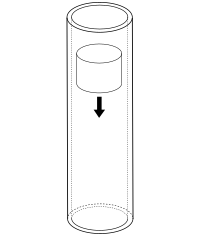
\includegraphics[width=0.7\textwidth]{./figures/movingmaxwell/magnet_falling.pdf}
\end{subfigure}
\begin{subfigure}[t]{0.49\linewidth}
    \centering
    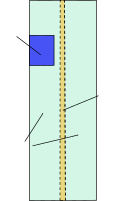
\includegraphics[width=0.5\textwidth]{./figures/movingmaxwell/magnet_falling_rz.pdf}
\end{subfigure}
\caption{磁体在铜管中下落过程示意图(左)及其 $rz$ 平面截面图(右).}
\label{fig:eddy_current}
\end{figure}
在此算例中,我们模拟一个物理实验现象,如图\ref{fig:eddy_current}所示,
一个圆柱形磁体自由下落进入垂直放置的铜管的过程。
根据法拉第电磁感应定律,磁体下落时在铜管中会感应出涡电流,
磁体的重力势能将转化为涡电流的电能,因此,磁体不会做自由落体运动,
其速度不会随着时间线性增加,而是逐渐趋于稳定。本算例使用的数据来自
文献 \cite{levin2006electromagnetic}:
铜管内半径为0.0785 m,壁厚为0.019 m,长度为0.8 m,电导率为\( 5.998 \times 10^7 \,
\text{S/m} \),磁导率为\( 4\pi \times 10^{-7} \, \text{H/m} \),
磁体半径为0.0635 m,高度为0.0635  m,
电导率为\( 7.14 \times 10^5 \, \text{S/m} \),
磁导率为\( 4\pi \times 10^{-7} \, \text{H/m} \),磁化强度
$\bm M = \dfrac{1.41}{4\pi \times 10^{-7}} \bm e_{z}$。
质量 $m = 0.006kg$,重力加速度 $g = 9.8 m/s^2$。
整个计算区域为 $\Omega = (0, 0.3) \times (0, 0.8)$。

在本实验中没有外加电流,
磁体运动过程中会受到两个力的作用,一个是重力 $\bF_g = -mg\be_z$,
另一个是涡电流产生的阻力 $\bF_e$,
其中阻力 $\bF_{e}$ 是铜管受到的洛伦兹力的反作用力,其大小为:
\begin{equation}
\label{eddy_current_force}
\bF_{e} = -\int_{\Omega_c} (\bJ \times \bB)\cdot\be_z \dd \bm x \be_z,
\end{equation}
其中 $\cdot \be_z$ 是轴对称的原因,$r$ 方向的力会抵消,仅受到 $z$ 方向的力。
磁体的运动方程为:
$$
\begin{aligned}
    m\frac{\dd \bu}{\dd t} & = \bF_{g} + \bF_{e},\\
\bu(0) & = 0.
\end{aligned}
$$
计算过程中,
根据虚单元方法 \eqref{vemaxial} 
获得第 $n$ 个时间层的磁矢势 $\bA^n_h = A^n_h\be_z$ 后,根据如下公式计算$\bB^n_h$ 和
$\bJ^n_h$:
$$
\bB^n_h = \bcurl \bA^n_h, \quad \bJ^n_h = \sigma\bE^n_h = -\sigma
\frac{A^n_h - A^{n-1}_h}{\tau}\be_{\theta}.
$$
然后根据公式\eqref{eddy_current_force}计算阻力 $\bF_{e}$,
最后 $\bu^n$ 通过以如下公式计算得到:
$$
\bu^n = \bu^{n-1} + \delta t \frac{\bF_{g} + \bF_{e}}{m}.
$$

图\ref{fig:eddy_current_result}展示了模拟过程中速度,
我们可以看到磁体的下落速度逐渐减小,然后趋于稳定,最终速度为
$6.2 cm/s$,
%这与文献\cite{levin2006electromagnetic}
%中的理论值 $7.3 cm/s$ 基本接近,
需要说明的是我们的结果与商业软件模拟结果完全一致。

\begin{figure}[H]
\centering
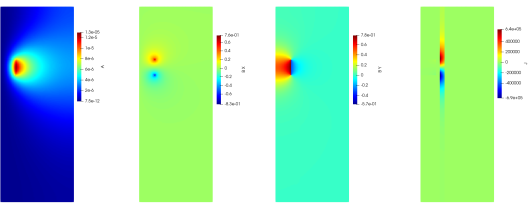
\includegraphics[width=0.8\textwidth]{./figures/movingmaxwell/ABXBYJ.pdf}
\caption{在 $0.03s$ 时磁矢势强度 $A$,磁感应强度 $\bB$ 的 $r$ 分量
和 $z$ 分量,以及涡电流密度 $J$ 的分布.}
\label{fig:eddy_current_result}
\end{figure}

\begin{figure}[H]
\begin{subfigure}[t]{0.49\linewidth}
    \centering
    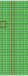
\includegraphics[width=0.3\textwidth]{./figures/movingmaxwell/mesh30.pdf}
\end{subfigure}
\begin{subfigure}[t]{0.49\linewidth}
    \centering
    \includegraphics[width=1.0\textwidth]{./figures/movingmaxwell/v.png}
\end{subfigure}
\caption{ 在 $0.03s$ 时的网格(左)与计算过程中磁体的速度随时间的变化(右).}
\end{figure}

%\subsection{电磁成型数值模拟}
%在此算例中,我们模拟了电磁成型过程,如图\ref{fig:emforming}所示的一个简化的模型,
%一个轴对称的工件和一个线圈,
%在线圈中通以交流电流,根据安培定律,
%线圈中的交流电流会产生交变磁场,从而在
%工件中会产生涡电流,工件在洛伦兹力的作用下产生形变。
%计算的参数来自与文献\CC{文献文献文献},
%工件的半径为 $0.055m$,高度为 $0.0012m$,
%电导率为 $2.59 \times 10^7 \, \text{S/m}$,密度为 $2700 \, \text{kg/m}^3$,
%线圈区域的内径为 $0.009m$,外径为
%$0.0339m$,线圈中施加的电流如图\ref{fig:emforming}所示。
%
%在实际的电磁成型过程中工件会产生大变形,
%需要对工件的形变进行建模,
%但这不是本文的重点,因此本实验中仅考虑
%工件的刚体运动,
%与前述的数值模拟过程相同,我们使用虚单元方法求解涡电流方程,
%并根据涡电流计算洛伦兹力,最后根据洛伦兹力计算工件的形变。
%在这种情况下,工件仅会沿 $z$ 方向移动。
%
%\begin{figure}[htpb]
%    \begin{subfigure}[t]{0.49\linewidth}
%        \centering
%        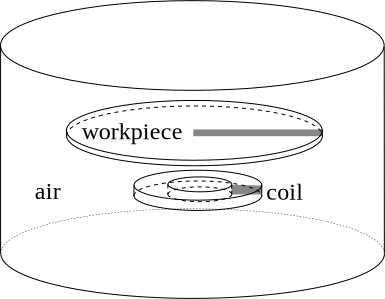
\includegraphics[width=0.7\textwidth]{./figures/movingmaxwell/EMF.pdf}
%    \end{subfigure}
%    \begin{subfigure}[t]{0.49\linewidth}
%        \centering
%        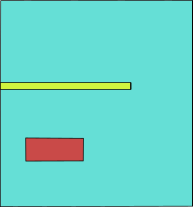
\includegraphics[width=0.5\textwidth]{./figures/movingmaxwell/emf_rz.pdf}
%    \end{subfigure}
%    \caption{电磁成型示意图(左)及其 $rz$ 平面剖面图(右)。}
%    \label{fig:emforming}
%\end{figure}





